\documentclass[12pt,letterpaper]{article}

\usepackage{amsmath}
\usepackage[pdftex]{graphicx}
\usepackage{hyperref} 

\parindent 0cm

\graphicspath{{figures/}}

\author{
    E. Jed Barlow\\
    \textit{ejbarlow@ualberta.ca}
}
\title{RpkmVisualizer Plugin Manual}

\begin{document}
\maketitle

\hfill

\tableofcontents

\newpage
\section{Overview}


RpkmVisualizer operates on the output of RNA-Seq to generate a circular bar
graph of RPKM values for regions of a genome.

\subsection{Intended Use}

The plugin is meant to be used as part of gene diversity and abundance analysis
of microbial populations.  The intended workflow involves assembling and
annotating a consensus sequence from DNA reads from a sample of a population,
and then using RNA-Seq on this sequence and the original set of DNA reads.
Though RNA-Seq is normally purposed for gene expression analysis, it is used
here for abundance analysis.  Among the resulting table is a column RPKM, which
stands for Reads Per Kilobase of exon model per Million mapped reads, and is a
measure representing the amount of reads per annotated region (gene).  The RPKM
values can then be used to infer the relative frequency of the presence of
genes in a population.  RpkmVisualizer serves to represent these findings
graphically by displaying the magnitude of the RPKM values for each region
along the genome.

\section{Installation}

\subsection{Downloading}

The plugin can be obtained from two locations.

\begin{itemize}
\item
    In source form: \url{http://github.com/jedbarlow/rpkmvisualizer}
\item
    As a compiled package: \url{http://www.ualberta.ca/~ejbarlow/biol498/}
\end{itemize}

\subsection{Loading into CLC Genomics Workbench}

Once obtained, the plugin \textit{rpkmvisualizer.cpa} can be installed as
follows.  First, click the \texttt{Plugins} button in the CLC Genomics
Workbench toolbar in the top-right corner of the main window.

\begin{center}
    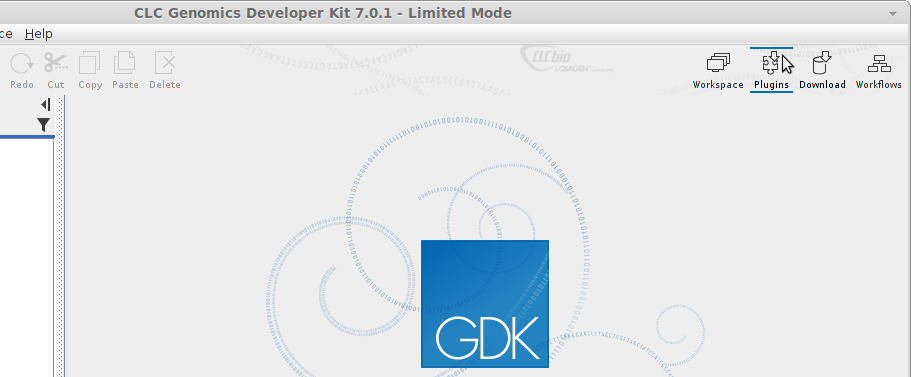
\includegraphics[width=34em]{plugins-button.png}
\end{center}

Then click the \texttt{Install From File} button.

\begin{center}
    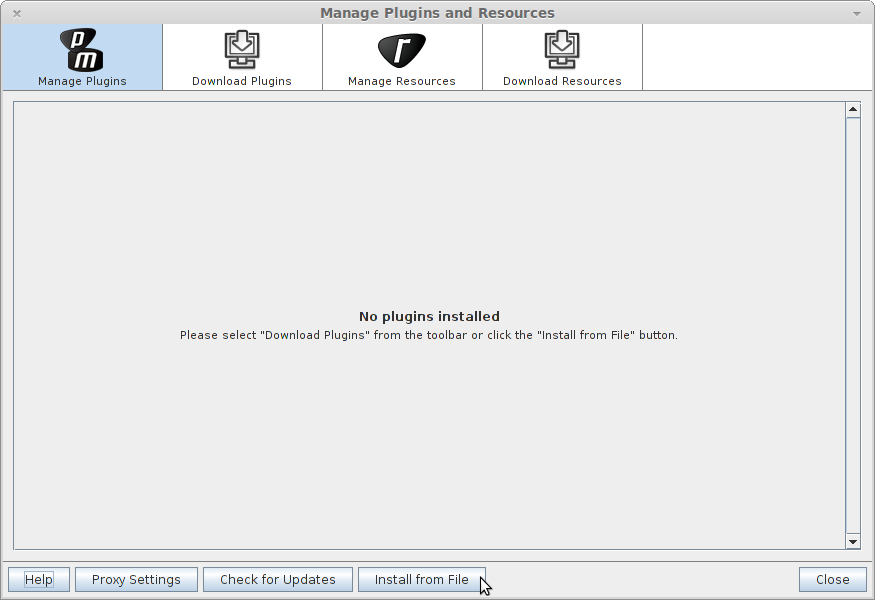
\includegraphics[width=34em]{install-from-file-button.png}
\end{center}

Then navigate to the folder containing the \texttt{rpkmvisualizer.cpa} file,
select the file, and click the \texttt{Install From File} button.

\begin{center}
    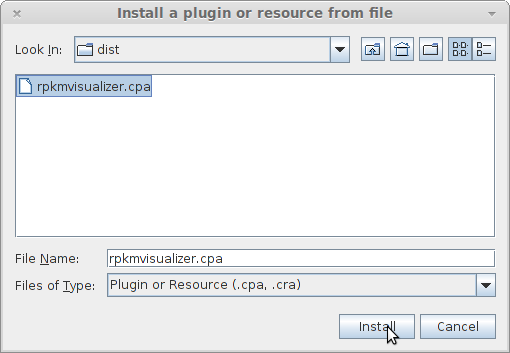
\includegraphics[width=26em]{install-button.png}
\end{center}

Then follow the on-screen steps of the wizard.  Once installed, \texttt{RPKM
Heat Map} should appear inside the \texttt{Show} viewing option in the
right-click menu as indicated by the figure in the next section below.

\section{Operation}

\subsection{Accessing the Plugin}

In the CLC Genomics Workbench explorer pane, right-click on the result table of
the RNA-Seq tool, and navigate to the \texttt{RPKM Heat Map} option as shown in
the following screenshot.

\begin{center}
    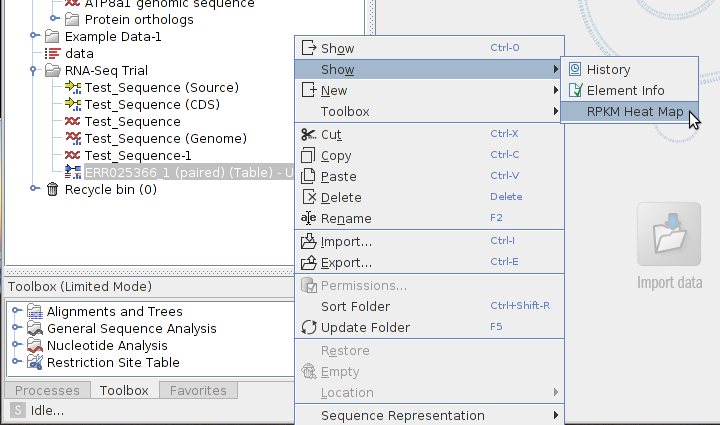
\includegraphics[width=34em]{access-plugin.png}
\end{center}

This will cause a view to be opened of the circular bar graph figure, similar
to the following example image.

\begin{center}
    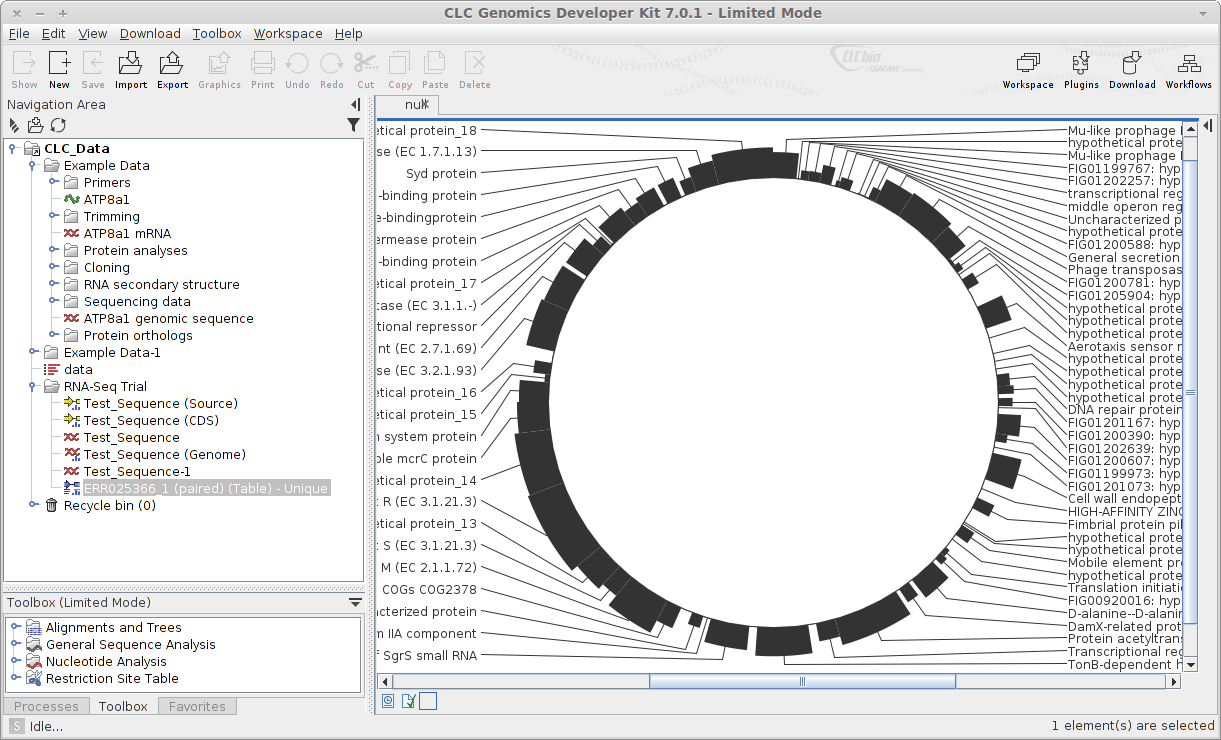
\includegraphics[width=32em]{plugin-result.png}
\end{center}

\subsection{Plugin Configuration}

A sidebar with options can be accessed by clicking the arrow near the top-right
corner of the figure, next to the vertical scrollbar.

\begin{center}
    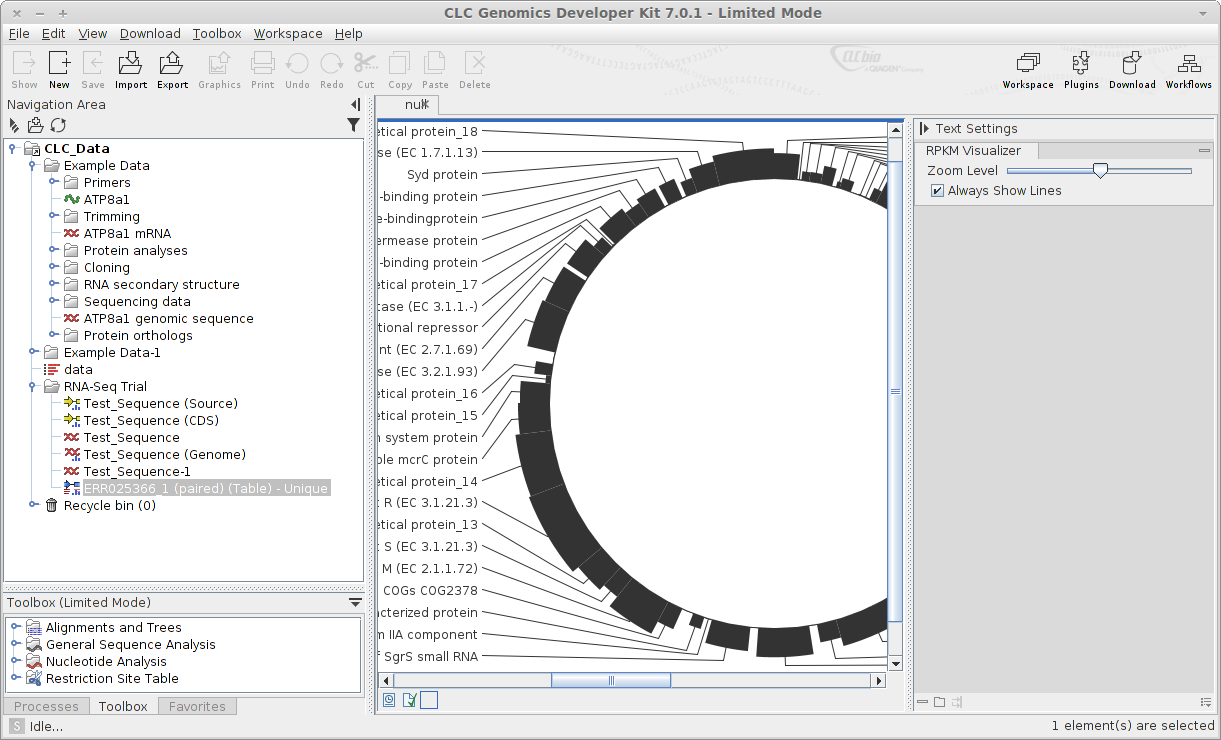
\includegraphics[width=32em]{sidebar.png}
\end{center}

These options can be used to adjust basic parameters of the figure, such as
zoom level and other layout options.  For example, the following image
demonstrates a change in zoom level and line visibility options.

\begin{center}
    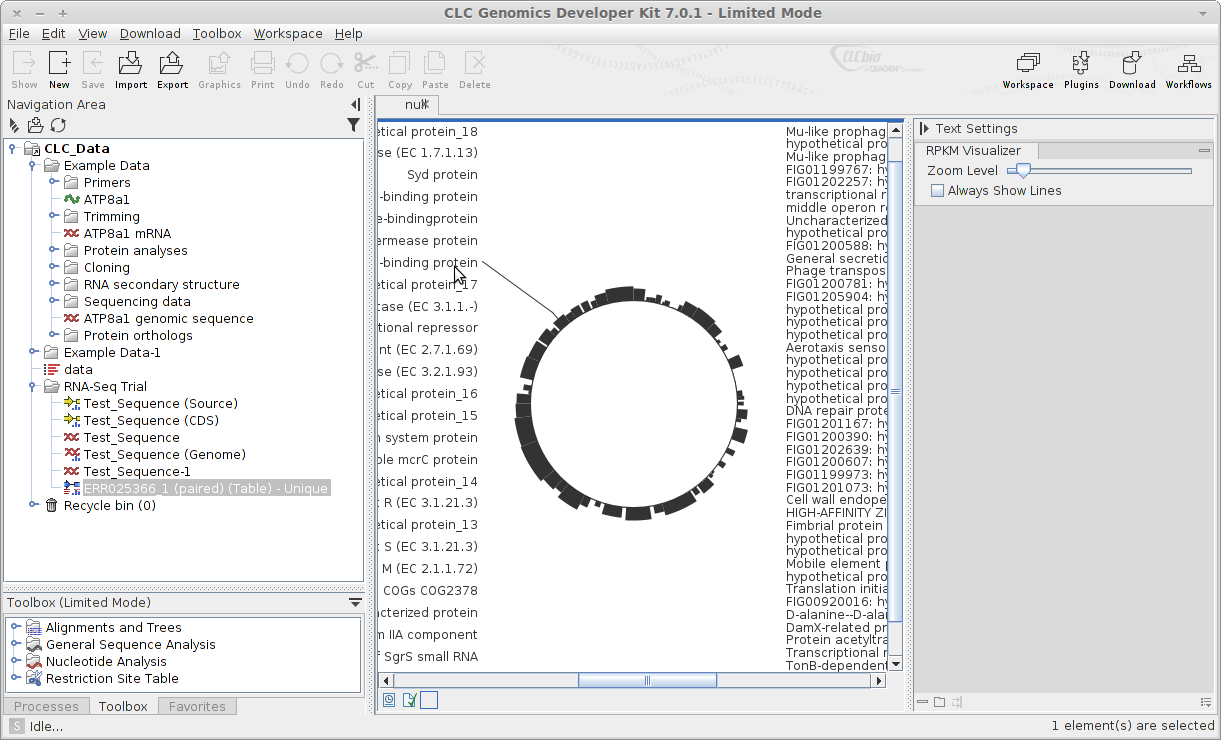
\includegraphics[width=32em]{sidebar-changed.png}
\end{center}

\section{Additional Information and URLs}

RpkmVisualizer is being actively developed by Jed Barlow at the Boucher Lab
(Department of Biological Sciences, University of Alberta) under the direction
of Yan Boucher.

\begin{itemize}
    \item
        Boucher Lab: \url{http://www.biology.ualberta.ca/boucher\_lab/Boucher\_Lab/Welcome.html}
\end{itemize}

\end{document}
